\chapter{AutoREST: Geração Automática de APIs REST para Funcionalidades CRUD}
\label{chap:autorest}

Neste capítulo, iremos apresentar a solução proposta para as questões levantadas neste estudo. A solução proposta, chamada AutoREST, é composta por um processo de modelagem de estruturas de dados e uma ferramenta de geração automática de APIs utilizando estes modelos como entrada. Serão apresentados os pontos motivadores deste estudo seguidos dos requisitos para a validação da solução proposta. Em seguida, a arquitetura AutoREST é proposta para cumprir com estes requisitos e, finalmente, a modelagem de uma instância desta arquitetura é apresentada como prova de conceito, utilizando as linguagens de modelagem UML e JSON Schema, o framework de programação Node.js e o sistema gerenciador de bancos de dados (SGBD) MongoDB através da biblioteca Mongoose.

%------------------------------------------------------------

\section{Motivação}

É parte essencial de sistemas Web que lidem com dados de persistência a implementação de APIs para a recepção e encaminhamento de requisições do tipo CRUD. Dentre as formas de implementação deste tipo de serviço o estilo arquitetural REST se destaca como a base fundamental da Internet e, portanto, é particularmente apropriada como base para o desenvolvimento de APIs de comunicação e acesso a recursos \cite{FIELDING:2000}.

A geração automática de código a partir de modelos é uma maneira de garantir a confiabilidade destas APIs e aumentar a produtividade do processo de geração de sistemas \cite{SELIC:2003}. Visto que a arquitetura REST tem entre suas restrições a presença de interfaces uniformes, com interações auto-contidas, a geração de APIs REST se apresenta particularmente bem para a aplicação de métodos de representação conceitual e geração de código automática.

O objetivo deste trabalho é a proposta de um paradigma para a representação conceitual do fornecimento de objetos por uma API REST, baseado na abordagem MDD. Além disso, buscamos uma maneira de proporcionar a geração automática de APIs REST para funcionalidades de manutenção de documentos de persistência a partir destes modelos conceituais, baseada na abordagem GP. Finalmente, a solução é apresentada utilizando modelos arquiteturais baseados nos preceitos da abordagem CBSE.

%------------------------------------------------------------

\section{Requisitos}
\label{sec:reqs}

Nesta seção, apresentamos os requisitos que foram identificados ao longo deste estudo para que o processo de modelagem conceitual e de geração automática de código para APIs REST seja possível. Foram levadas fortemente em consideração as metodologias apresentadas no Capítulo \ref{chap:modelagem} e os padrões arquiteturais apresentados no Capítulo \ref{chap:arquitetura}. Estes requisitos foram formulados para servir como base para o projeto de uma arquitetura de software altamente independente de tecnologias de implementação.

\begin{itemize}
    \item RQ01: A solução apresentada deve proporcionar orientações exatas para a modelagem conceitual de uma estrutura de dados contendo todas as entidades, associações, atributos e restrições de integridade necessárias para a geração automática de uma API REST. Este modelo conceitual deve utilizar de linguagem gráfica que seja considerada de fácil compreensão e manutenção pela literatura de referência, conforme preceitos da abordagem MDD;
    \item RQ02: O sistema deve ser capaz de converter um modelo conceitual criado em linguagem gráfica para uma estrutura intermediária de fácil processamento por máquinas. Esta estrutura deve conter todos os dados presentes no modelo conceitual original;
    \item RQ03: O sistema deve gerar automaticamente, a partir de um modelo conceitual conforme RQ01, uma API REST que implemente as operações básicas de manutenção das entidades componentes do esquema conceitual (CRUD). Esta geração deve se valer de blocos de código parametrizáveis para a padronização das APIs geradas, conforme preceitos da abordagem GP;
    \item RQ04: O código fonte gerado deverá ser implementado de forma a permitir a persistência e manipulação dos recursos acessados durante a operação da API REST através de um SGBD;
    \item RQ05: A arquitetura da solução deverá se valer de interfaces com contratos bem definidos de forma a permitir a implementação de novos componentes para a extensão da aplicação, conforme preceitos da abordagem CBSE.
\end{itemize}

%------------------------------------------------------------

\section{Decisões de Projeto}
\label{sec:dds}

Nesta seção são apresentadas as decisões de projeto referentes a uma instância da arquitetura AutoREST, que será projetada e desenvolvida como prova de conceito da arquitetura e como embasamento para responder as perguntas de pesquisa propostas nesse trabalho. Estas decisões de projeto foram desenvolvidas com base nas tecnologias e linguagens apresentadas no Capítulo \ref{chap:tecno}.

\begin{itemize}
    \item DD01 (referente ao RQ01): Serão criadas orientações para a modelagem de um Diagrama de Classes UML da ferramenta Astah para servir como modelo de configuração. Este diagrama irá representar um esquema conceitual de dados sobre a qual a API REST será gerada, com suas classes, relacionamentos, atributos e domínios, e anotado com um subconjunto da linguagem JSON Schema para representar as restrições de integridade das entidades.
    \item DD02 (referente ao RQ02): O sistema irá dispor de algoritmos e regras de conversão de um Diagrama de Classes UML anotado conforme DD01 para uma representação de definições JSON Schema, que irá servir como PFIS (Processing-Friendly Intermediate Structure) do sistema.
    \item DD03 (referente ao RQ03): O sistema irá realizar a geração automática de uma API REST em código na linguagem Node.js a partir das definições JSON Schema geradas conforme DD02. Este código deverá desempenhar as operações básicas de manutenção de documentos de persistência (CRUD).
    \item DD04 (referente ao RQ04): A API REST gerada irá persistir os dados através do SGBD MongoDB, utilizando-se da biblioteca Mongoose.
    \item DD05 (referente ao RQ03): O sistema irá realizar a geração de código a partir de fragmentos de código pré-implementados representando cada um dos métodos HTTP (GET, HEAD, POST, PUT, PATCH, DELETE).
    \item DD06 (referente ao RQ05): O sistema será desenvolvido em quatro partes independentes, como representadas na Figura \ref{fig_aba}, sendo estas: um leitor de arquivos XML representativos de Diagramas de Classes UML da ferramenta Astah, conforme DD01; um conversor de Diagramas de Classes UML anotados para definições em JSON Schema, conforme DD02; um gerador de código Node.js para APIs REST a partir de definições JSON Schema, conforme DD03, e; um componente de interface com usuário e controle de execução de sistema.
\end{itemize}

%------------------------------------------------------------

\section{Proposta de Solução}

Para que todos os requisitos apresentados acima sejam cumpridos, é proposto o modelo arquitetural AutoREST, uma arquitetura independente de tecnologia, com seus modelos estruturais e comportamentais em linguagem UML. Exemplos de possíveis concretizações dos componentes conceituais são apresentadas para motivos de contextualização.

Projetada com base nos preceitos da abordagem CBSE, utilizando como domínio de solução as aplicações para a geração automática de APIs REST a partir de esquemas conceituais, a AutoREST é composta de quatro subsistemas na forma de componentes que operam de forma autônoma e cinco interfaces de comunicação para permitir a cooperação entre estes quatro subsistemas. Cada subsistema possui uma dependência ligada às interfaces ao qual está relacionado, mas se mantém independente dos outros subsistemas. Desta forma, a arquitetura obedece o requisito RQ05 listado na Seção \ref{sec:reqs}.

\begin{figure}[htb]
    \begin{center}
        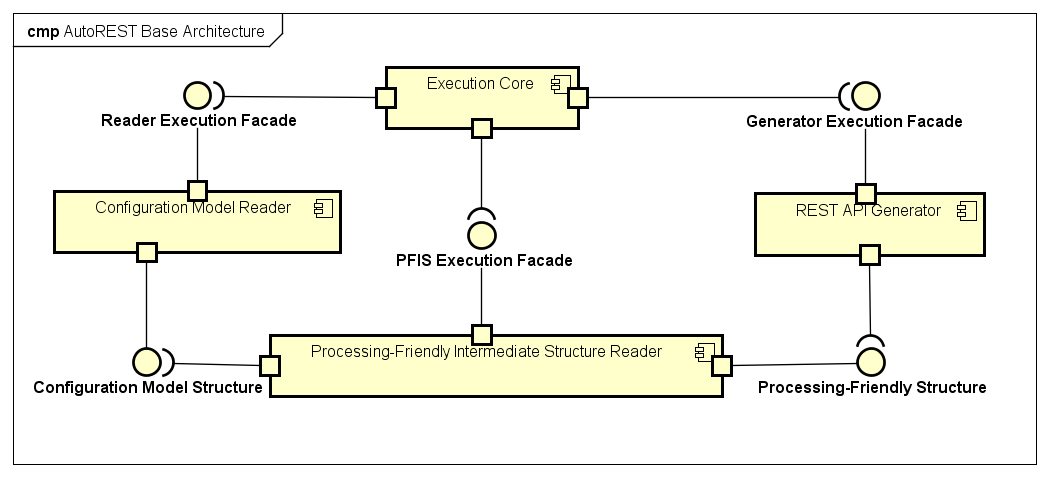
\includegraphics[scale=0.57]{imagens/AutoREST_Base_Architecture.png}
    \end{center}
	\caption{\label{fig_aba}AutoREST - Arquitetura Base}
\end{figure}

A Figura \ref{fig_aba} apresenta um diagrama de componentes UML representando os quatro subsistemas e suas interfaces. As seções a seguir descrevem cada um destes subsistemas e interfaces em maior detalhe.

\begin{itemize}
    \item \textit{Execution Core}: é o subsistema encarregado de controlar a execução da ferramenta, provendo as interfaces de usuário e gerenciando a comunicação dos outros subsistemas;
    \item \textit{Configuration Model Reader} (CMR): é o subsistema encarregado da leitura do modelo conceitual em linguagem gráfica, criado conforme orientações dadas pela documentação do componente utilizado na implementação da arquitetura;
    \item \textit{Processing-Friendly Intermediate Structure Reader} (PFIS-R): é o subsistema encarregado de realizar a tradução do modelo conceitual em linguagem gráfica para uma estrutura intermediária de fácil processamento;
    \item \textit{REST API Generator}: é o subsistema encarregado da geração de uma implementação da API REST representada no esquema conceitual de entrada do sistema;
    \item \textit{Execution Facades}: são as interfaces utilizadas para a comunicação do subsistema de controle com os outros subsistemas e definidas utilizando o padrão de projeto Fachada \cite{GAMMA:1995};
    \item \textit{Configuration Model Structure}: é a interface de comunicação entre os subsistemas CMR e PFIS-R, servindo como ponto de transferência do modelo conceitual em linguagem gráfica entre os dois subsistemas;
    \item \textit{Processing-Friendly Structure}: é a interface de comunicação entre os subsistemas PFIS-R e \textit{REST API Generator}, servindo como ponto de transferência da estrutura intermediária de fácil processamento entre os dois subsistemas.
\end{itemize}

%------------------------------------------------------------

\subsection{\textit{Execution Core} e \textit{Execution Facades}}

O subsistema \textit{Execution Core} é responsável pelo controle da aplicação através de requisições às \textit{Execution Facades}. Estas requisições devem ser procedimentos ativadores das funções básicas de cada um dos subsistemas, transferindo pacotes de dados entre eles. Estes pacotes de dados serão estruturados conforme as interfaces providas pelos subsistemas CMR, PFIS-R e Generator.

\begin{figure}[htb]
    \begin{center}
        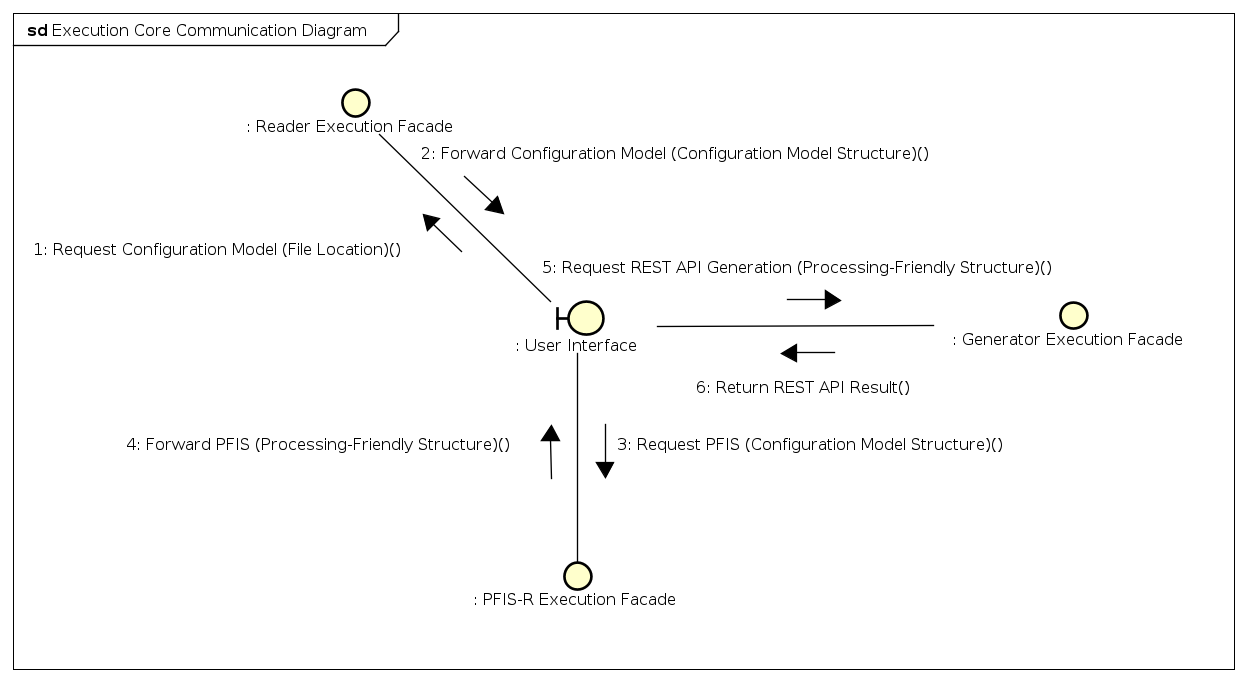
\includegraphics[scale=0.57]{imagens/Execution_Core_Communication_Diagram.png}
    \end{center}
	\caption{\label{fig_eccom}Diagrama de Comunicação do Subsistema \textit{Execution Core}}
\end{figure}

A Figura \ref{fig_eccom} apresenta um diagrama de comunicação entre a interface de usuário provida pelo \textit{Execution Core} e as interfaces de \textit{Execution Facade}. A comunicação ocorre através de seis mensagens básicas:

\begin{enumerate}
    \item É realizada uma requisição ao \textit{Reader Execution Facade} para que o modelo conceitual, contido em um arquivo cuja localização é enviada como argumento, seja carregado em memória;
    \item Após a execução dos processos internos do subsistema CMR, o modelo conceitual é retornado ao \textit{Execution Core} para que este dê continuidade ao processo;
    \item É realizada uma requisição ao \textit{PFIS-R Execution Facade} para que o modelo conceitual em memória, contido em um pacote de dados enviado como argumento, seja convertido em uma PFIS;
    \item Após a execução dos processos internos do subsistema PFIS-R, a PFIS é retornada ao \textit{Execution Core} para que este dê continuidade ao processo;
    \item É realizada uma requisição ao \textit{Generator Execution Facade} para que a API REST seja gerada a partir do PFIS em memória, contido em um pacote de dados enviado como argumento;
    \item O código gerado é retornado ao \textit{Execution Core} e entregue ao usuário.
\end{enumerate}

O resultado da composição do sistema através deste padrão de comportamento é um desacoplamento dos outros subsistemas componentes da arquitetura AutoREST, permitindo que estes sejam construídos de forma semi-autônoma, tendo como dependência apenas as estruturas de dados providas por interfaces de outros subsistemas.

%------------------------------------------------------------

\subsection{\textit{Configuration Model Reader} (CMR) e \textit{Configuration Model Structure}}
\label{sec:cmr}

O subsistema \textit{Configuration Model Reader} (CMR) é responsável por definir a estrutura interna de sistema do modelo de configuração (representado por um modelo conceitual em linguagem gráfica) da ferramenta AutoREST. Além disto, é responsável por prover as funcionalidades de IO relacionadas a estes modelos. Este subsistema é composto de elementos de código e artefatos de documentação, visto que é parte dele também a definição de orientações e restrições para a construção dos modelos de configuração, conforme RQ01 apresentada na Seção \ref{sec:reqs}.

Minimamente, a estrutura de dados definida pelo subsistema CMR deve conter representações de entidades com identificadores únicos, associações entre estas entidades, seus atributos e suas restrições de integridade. Exemplos de linguagens de modelagem que proveem estes elementos são Diagramas de Classes UML anotados (utilizado na prova de conceito apresentada na Seção \ref{sec:conceptproof}) e Modelos Entidade-Relacionamento \cite{POLAK:2015} \cite{VALVERDE:2009}.

Algumas restrições de integridade que se mostraram importantes na representação de uma RESTful API são: restrições de tipo de atributos, tipos de acesso aceitos para cada associação, notação de mandatório ou multiplicidade e notação de herança. Em relação à questão de tipos de acesso aceitos por associação, se quer dizer especificamente quais os atributos que podem ser utilizados em requisições HTTP a partir das entidades que compõe a associação.

Nosso estudo não identificou utilidade prática de determinadas restrições de integridade na geração de RESTful APIs. São estas: notações de classes internas, modificadores de acesso, entidades com identificadores compostos (aridade maior do que um) e atributos com tipos de dado não primitivos. Também não conseguimos identificar uma forma de implementar associações sem atributo relacionado, visto que todo recurso REST deve ser acessado através de um identificador.

%------------------------------------------------------------

\subsection{\textit{Processing-Friendly Intermediate Structure Reader} (PFIS-R) e \textit{Processing-Friendly Structure}}

O subsistema \textit{Processing-Friendly Intermediate Structure Reader} (PFIS-R) é responsável pela tradução do modelo de configuração em um modelo textual equivalente para fácil processamento no estágio de geração da API REST, no subsistema \textit{REST API Generator}. Este subsistema é composto por três componentes como representado na Figura \ref{fig_pfisrcom}.

\begin{figure}[htb]
    \begin{center}
        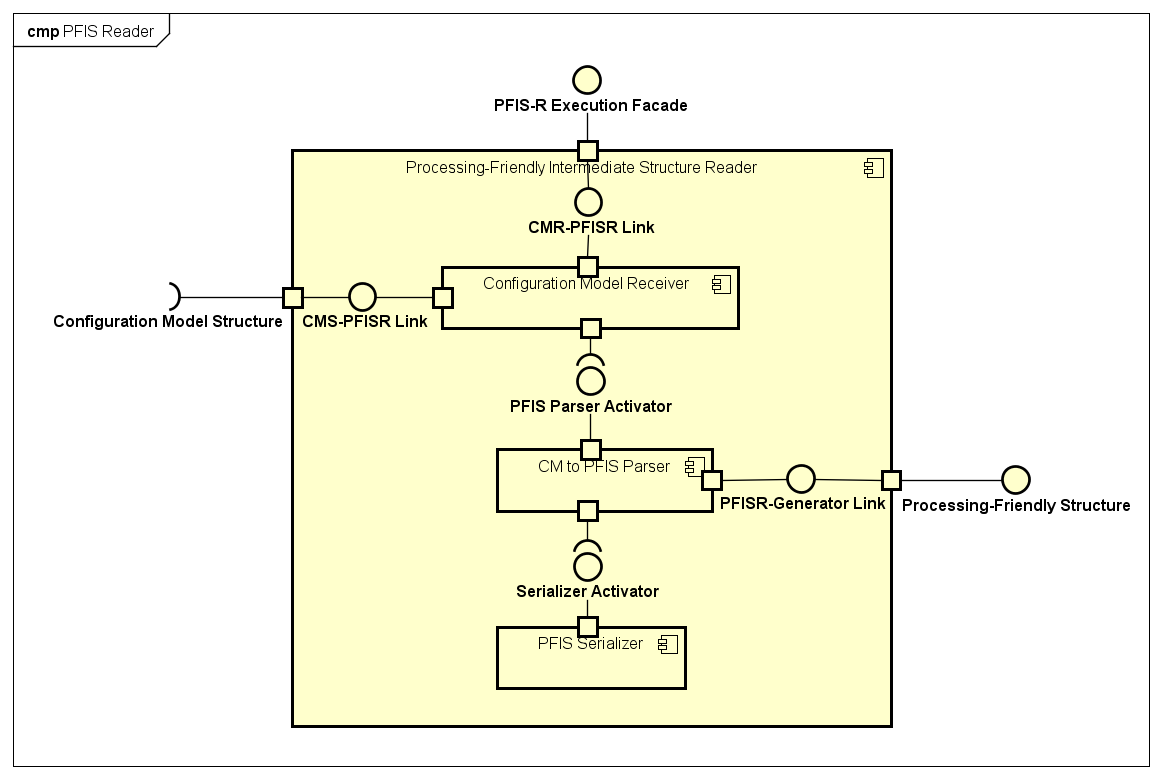
\includegraphics[scale=0.52]{imagens/PFIS_Reader_Subcomponent_Diagram.png}
    \end{center}
	\caption{\label{fig_pfisrcom}Diagrama de Componentes do Subsistema PFIS-R}
\end{figure}

As interfaces internas do subsistema, que realizam a comunicação entre os componentes, permitem um grau de autonomia entre os componentes do subsistema PFIS-R. A execução deste subsistema é descrita pelo Diagrama de Sequência apresentado nas Figuras \ref{fig_pfisrseq1} e \ref{fig_pfisrseq2}. A interface CMS-PFISR Link é omitida para reduzir o tamanho da figura.

\begin{figure}[htb]
    \begin{center}
        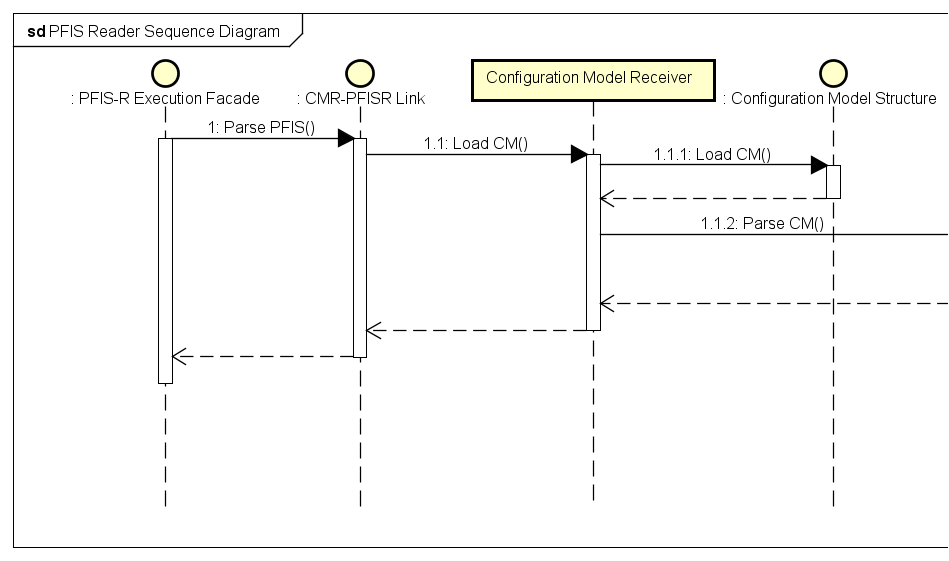
\includegraphics[scale=0.57]{imagens/PFIS_Reader_Sequence_Diagram_1.png}
    \end{center}
	\caption{\label{fig_pfisrseq1}Diagrama de Sequência do Subsistema PFIS-R - Parte 1}
\end{figure}

\begin{figure}[htb]
    \begin{center}
        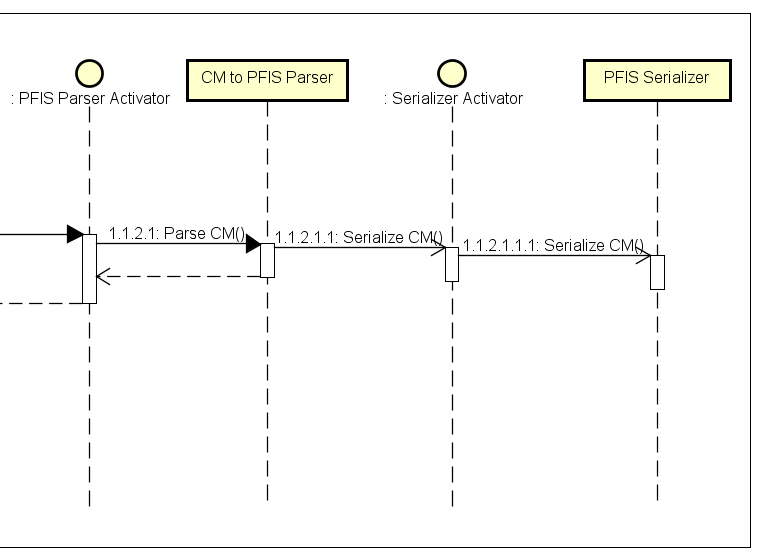
\includegraphics[scale=0.59]{imagens/PFIS_Reader_Sequence_Diagram_2.png}
    \end{center}
	\caption{\label{fig_pfisrseq2}Diagrama de Sequência do Subsistema PFIS-R - Parte 2}
\end{figure}

Este subsistema também é responsável por definir a estrutura interna de sistema da PFIS. Esta representação deve ser feita através de uma linguagem textual bem definida por terceiros, em conformidade com as definições de CBSE de \citeonline{JIFENG:2005}. Também é importante ressaltar mais uma vez que deve haver equivalência entre as representações CM e PFIS. Exemplos de linguagens que podem ser utilizadas para esta representação são RAML \cite{RAML}, Swagger \cite{SWAGGER}, WSDL \cite{BOOTH:2005} e JSON Schema \cite{PEZOA:2016}, este último sendo utilizado na prova de conceito apresentada na Seção \ref{sec:conceptproof}.

%------------------------------------------------------------

\subsection{\textit{REST API Generator}}

O subsistema \textit{REST API Generator} é responsável pela fase final da operação de um sistema AutoREST: a geração do código fonte de uma API REST. Este subsistema é composto por dois componentes, como apresentado na Figura \ref{fig_gencomp}: \textit{PFIS Compiler} e \textit{HTTP Method Stub Library}. O \textit{PFIS Compiler} é responsável pela execução deste subsistema, recebendo requisições através da interface \textit{Generator Execution Facade} e realizando a leitura de uma PFIS através da interface provida pelo subsistema PFIS-R.

\begin{figure}[htb]
    \begin{center}
        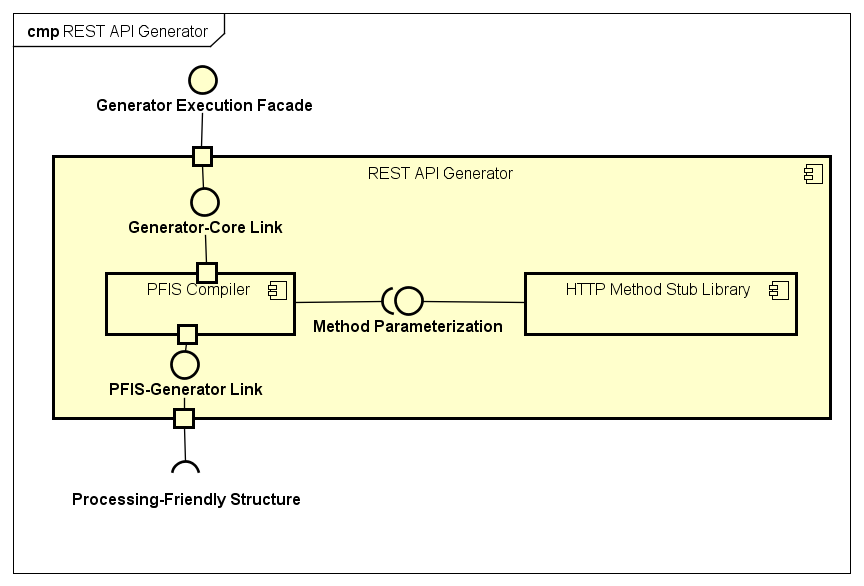
\includegraphics[scale=0.65]{imagens/REST_API_Generator_Subcomponent_Diagram.png}
    \end{center}
	\caption{\label{fig_gencomp}Diagrama de Componentes do Subsistema \textit{REST API Generator}}
\end{figure}

A partir da leitura de uma PFIS, o subsistema realiza a geração de uma API REST baseada no código parametrizável implementado na \textit{HTTP Method Stub Library}, que serve como base para todas as APIs REST geradas por uma implementação deste subsistema, oferecendo código fonte base em determinada linguagem de programação. A forma utilizada para a leitura dos artefatos de entrada pelo gerador pode variar entre implementações, o que motivou a estruturação deste subsistema de forma a permitir o reuso de uma mesma \textit{HTTP Method Stub Library} em diversas implementações deste subsistema.

%------------------------------------------------------------

\section{Prova de Conceito - Instanciando a Arquitetura AutoREST}
\label{sec:conceptproof}

Como prova de conceito da arquitetura AutoREST, foi desenvolvido um sistema de geração de APIs REST baseado na arquitetura proposta\footnote{Disponível em \url{https://autorest-site.herokuapp.com/}}, conforme as decisões de projeto delineadas na Seção \ref{sec:dds}. Este sistema utiliza as tecnologias de Diagramas de Classes UML, JSON Schema, Java, Node.js e MongoDB.

Os componentes de sistema foram implementados na linguagem de programação Java, com exceção do subsistema Execution Core, que foi desenvolvido em JavaScript. Cada um dos subsistemas foi implementado de forma autônoma, e suas interações são realizadas através de arquivos, garantindo o cumprimento da RQ05.

A notação utilizada para modelos de configuração foi a de Diagramas de Classes UML anotados conforme Subseção \ref{sec:xmi}, utilizando um subconjunto da linguagem JSON Schema conforme a definição de \citeonline{PEZOA:2016}. O artefato de entrada do subsistema instância de \textit{Configuration Model Reader} é um XML gerado pela ferramenta Astah. A utilização de UML como linguagem gráfica para o modelo de configuração garante o cumprimento da RQ01 \cite{OMG:2011}.

A notação utilizada como PFIS foi um conjunto de definições JSON Schema, conforme Subseção \ref{sec:bnf} \cite{PEZOA:2016}. Este modelo é gerado automaticamente pelo sistema a partir do modelo de configuração, garantindo o cumprimento da RQ02.

A API REST é gerada utilizando a linguagem Node.js. Um compilador foi criado utilizando a ferramenta BYACC/J \cite{BYACCJ}, utilizando chamadas de função a uma biblioteca que contém blocos de código parametrizáveis representando os métodos HTTP. Além disto, a API REST fará uso da biblioteca Mongoose para permitir a persistência de objetos a partir do SGBD MongoDB. Desta forma, é garantido o cumprimento das RQ03 e RQ04.

%------------------------------------------------------------

\subsection{Modelo de Configuração - Orientações de Modelagem}
\label{sec:xmi}

Para que seja possível a conversão automática de um modelo de configuração, é necessário que este tenha uma notação formal estabelecida de acordo com regras específicas (conforme Seção \ref{sec:cmr}). Nesta seção serão apresentadas as orientações para a modelagem de um Diagrama de Classes UML anotado, utilizando a ferramenta Astah, para que este sirva como modelo de configuração para a ferramenta AutoREST implementada como prova de conceito. O uso de JSON Schema é majoritariamente baseado em \citeonline{DROETTBOOM:2015} e \citeonline{PEZOA:2016}. Todas as Regras de Modelagem serão indexadas como ``RM\#\#'' e as Regras de Conversão serão indexadas como ``RC\#\#''. A quebra de qualquer uma das RMs definidas nesta seção invalida o resultado da execução da ferramenta AutoREST implementada como prova de conceito, visto que implica na não-conformidade com um pré-requisito do uso da ferramenta.

%------------------------------------------------------------

\subsubsection{Classe e Atributos}

Um modelo simples que pode ser utilizado como exemplo é uma única classe, sem associações, contendo apenas atributos não anotados. A Figura \ref{fig_example_class} apresenta uma classe contendo atributos de todos os tipos que são suportados pela ferramenta.

\begin{figure}[htb]
    \begin{center}
        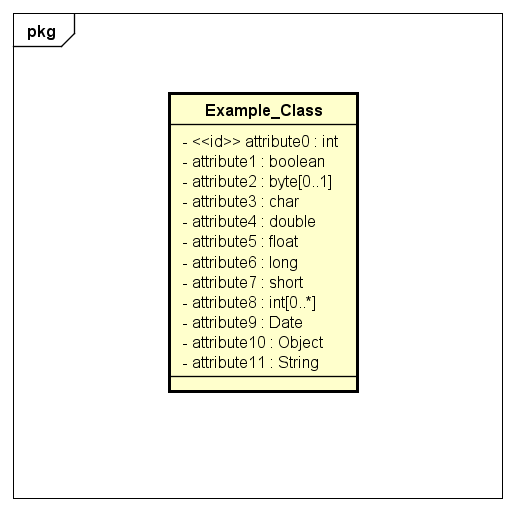
\includegraphics[scale=0.7]{imagens/Example_Class.png}
    \end{center}
	\caption{\label{fig_example_class}Classe UML - Astah}
\end{figure}

Esta classe contém doze atributos numerados de 0 a 11, sendo o primeiro (\textit{attribute0}) o identificador da classe. As seguintes regras de modelagem são estabelecidas a partir desta figura:

\begin{itemize}
    \item RM01: Todo elemento Classe deve ter um nome único dentro do escopo do diagrama, maior do que um caractere, sem espaços (utilizar CamelCase ou \_underscore).

    \item RM02: Todo elemento Classe deve ter um e apenas um atributo identificado com o Esteriótipo <<id>>, representando o atributo identificador da classe. Caso nenhum atributo seja identificado com este esteriótipo, um atributo identificador será gerado pela ferramenta AutoREST durante a conversão para JSON Schema.

    \item RM03: Todo elemento Atributo deve ter um nome único dentro do escopo da classe, maior do que um caractere, sem espaços (utilizar CamelCase ou \_underscore).

    \item RM04: A visibilidade (modificador de acesso) de um elemento Atributo será ignorado pela ferramenta, e portanto pode ser demarcado com quaisquer opções disponíveis.

    \item RM05: Um elemento Atributo pode assumir os seguintes tipos: \textit{int}; \textit{boolean}; \textit{byte}; \textit{char}; \textit{double}; \textit{float}; \textit{long}; \textit{short}; \textit{Date}; \textit{Object}, e; \textit{String}. Também pode ser assumido como tipo quaisquer outras Classes disponíveis no diagrama. Os tipos \textit{double} e \textit{float} serão considerados como o mesmo tipo; da mesma forma, os tipos \textit{int}, \textit{long} e \textit{short} serão considerados como o mesmo tipo.

    \item RM06: Um elemento Atributo com multiplicidade 0..1 será considerado como opcional.

    \item RM07: Um elemento Atributo com multiplicidade diferente de 0..1 ou 1 será considerado um vetor do tipo especificado, tal que o primeiro valor representa o tamanho mínimo do vetor (utilizar 0 para valor mínimo não definido) e o segundo valor representa o valor máximo do vetor (utilizar * para valor máximo não definido).
\end{itemize}

A partir destas regras de modelagem, podem ser estabelecidas as seguintes regras de conversão para notação JSON Schema, utilizada como PFIS:

\begin{itemize}
    \item RC01: Cada elemento Classe será convertido em um elemento de tipo \textit{object} no campo \textit{definitions}, com o mesmo nome da Classe em questão.

    \item RC02: Cada elemento Atributo será convertido em um elemento no campo \textit{properties} da classe relacionada, com o mesmo nome do Atributo em questão.

    \item RC03: Atributos de tipo \textit{int}, \textit{short}, \textit{long} e \textit{byte} serão representados pelo tipo \textit{integer}. Adicionalmente, Atributos de tipo \textit{byte} serão marcados com as restrições de integridade de valor mínimo 0 e valor máximo 255.

    \item RC04: Atributos de tipo \textit{boolean} mantém o mesmo tipo na representação em PFIS.

    \item RC05: Atributos de tipo \textit{char}, \textit{String} e \textit{Date} serão representados pelo tipo \textit{string}. Adicionalmente, atributos de tipo \textit{char} serão marcados com a restrição de integridade de tamanho máximo 1, e atributos de tipo \textit{Date} serão marcados com a restrição de integridade \textit{``pattern'' : ``\^{}\textbackslash{}d\textbackslash{}d\textbackslash{}d\textbackslash{}d-(0?[1-9]\textbar{}1[0-2])-(0?[1-9]\textbar{}[12][0-9]\textbar{}3[01]) (00\textbar{}[0-9]\textbar{}1[0-9]\textbar{}2[0-3]):([0-9]\textbar{}[0-5][0-9]):([0-9]\textbar{}[0-5][0-9])\textdollar{}''} \footnote{Esta funcionalidade, apesar de especificada, não foi implementada na ferramenta prova de conceito.}.
    %^\d\d\d\d-(0?[1-9]|1[0-2])-(0?[1-9]|[12][0-9]|3[01]) (00|[0-9]|1[0-9]|2[0-3]):([0-9]|[0-5][0-9]):([0-9]|[0-5][0-9])$

    \item RC06: Atributos de tipo \textit{Object} ou atributos tipados com outras Classes disponíveis no diagrama serão representados pelo tipo JSON Schema \textit{object}. Adicionalmente, atributos tipados com outras Classes disponíveis no diagrama terão como propriedade a referência da definição da respectiva Classe.

    \item RC07: Todos os atributos serão definidos como dependentes do atributo identificador.

    \item RC08: Atributos com multiplicidade mínima maior do que 0 serão definidos como requeridos.

    \item RC09: Atributos com multiplicidade máxima maior do que 1 serão definidos como vetores.
\end{itemize}

%------------------------------------------------------------

\subsubsection{Restrições de integridade de atributos}

Restrições de integridade de atributos devem ser anotados diretamente nos atributos com a utilização de \textit{tags} no formato JSON Schema. Todas as restrições de integridade aqui definidas seguem a semântica definida por \citeonline{PEZOA:2016}. As restrições de integridade válidas são ditadas pelas regras de construção a seguir:

\begin{itemize}
    \item RM08: Atributos de tipos \textit{int}, \textit{short} e \textit{long} podem ser anotados com as \textit{tags}: \textit{min}, \textit{max}, \textit{exMin} e \textit{exMax}.

    \item RM09: Atributos de tipo \textit{byte} e \textit{Date} não podem ser anotados, tendo em vista que estes tipos já consideram restrições de integridade próprias.

    \item RM10: Atributos de tipo \textit{boolean} não podem ser anotados, dada a natureza primitiva deste tipo.

    \item RM11: Atributos de tipo \textit{char} e \textit{String} podem ser anotados com a \textit{tag}: \textit{pattern}. Adicionalmente, atributos de tipo \textit{String} também podem ser anotados com as \textit{tags}: \textit{minLength} e \textit{maxLength}.

    \item RM12: Atributos de tipo \textit{Object} não podem ser anotados, e servem como \textit{wildcard}. Para definições de objetos mais complexos, utilizar elementos do tipo Classe.

    \item RM13: Atributos tipados com outras Classes disponíveis no diagrama não podem ser anotadas, visto que estes atributos farão referência às restrições de integridade da Classe referenciada.

    \item RM14: Atributos com multiplicidade diferente de 0..1 ou 1 (tipo vetor) podem ser anotados com a \textit{tag}: \textit{uniqueItems}, de valor booleano (\textit{true} ou \textit{false}), representando a restrição de que todos os itens do vetor sejam diferentes entre si.
\end{itemize}

Estas \textit{tags} serão convertidas diretamente para as restrições de integridade equivalentes em JSON Schema, gerando uma única regra de conversão:

\begin{itemize}
    \item RC10: Todas as \textit{tags} de elementos do tipo Atributo serão convertidas em suas respectivas restrições de integridade JSON Schema \footnote{Esta funcionalidade, apesar de especificada, não foi implementada na ferramenta prova de conceito.}.
\end{itemize}

A Figura \ref{fig_example_tags} apresenta a parte da tela do Astah referente às \textit{tags}, com anotações referentes ao \textit{attribute11} da classe representada na Figura \ref{fig_example_class}.

\begin{figure}[htb]
    \begin{center}
        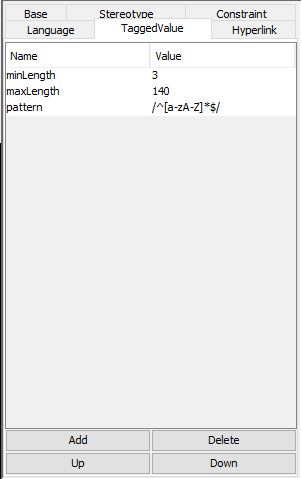
\includegraphics[scale=0.7]{imagens/Example_Tags.png}
    \end{center}
	\caption{\label{fig_example_tags}\textit{Tags} relativas ao \textit{attribute11} da Figura \ref{fig_example_class} - Astah}
\end{figure}

A partir das regras de conversão apresentadas até este ponto, a Classe representada na Figura \ref{fig_example_class} terá o formato em JSON Schema apresentado no Anexo \ref{fig_example_class_j}.

%------------------------------------------------------------

\subsubsection{Multiplicidade de Associações e Navegabilidade}

Associações simples entre duas classes podem ser representadas utilizando as notações de multiplicidade e navegabilidade. As restrições descritas nesta seção são detalhadas conforme \citeonline{BOOCH:2005}.

\begin{itemize}
    \item RM15: Associações podem ser navegáveis ou não-navegáveis. Associações anotadas como tendo navegabilidade não-definida serão considerados não-navegáveis.

    \item RM16: Associações podem ter multiplicidade 1, 0..1, 0..*, 1..* ou *. Associações de multiplicidade não definida serão consideradas como tendo multiplicidade 1.

    \item RM17: Vértices não-navegáveis de associações são considerados como tendo multiplicidade 1, independentemente da multiplicidade anotada no diagrama.
\end{itemize}

A partir destas regras de modelagem, podem ser estabelecidas as seguintes regras de conversão para PFIS (um vértice é considerado como tendo a mesma navegabilidade e multiplicidade da ponta oposta de uma associação na qual está relacionado):

\begin{itemize}
    \item RC11: Classes localizadas em vértices não-navegáveis não terão referência à classe associada.

    \item RC12: Classes localizadas em vértices navegáveis terão referência à classe associada conforme multiplicidade do vértice.

    \item RC13: Vértices de multiplicidade 1 ou 0..1 serão representados por uma referência ao atributo identificador da classe associada à sua especificação. Adicionalmente, vértices de multiplicidade 0..1 terão este atributo identificador representado como opcional.

    \item RC14: Vértices de multiplicidade 0..*, * ou 1..* serão representados por um vetor de referências ao atributo identificador da classe associada à sua especificação. Adicionalmente, vértices de multiplicidade 1..* terão adicionada a este vetor a restrição de integridade de tamanho mínimo 1.
\end{itemize}

\begin{figure}
    \begin{center}
        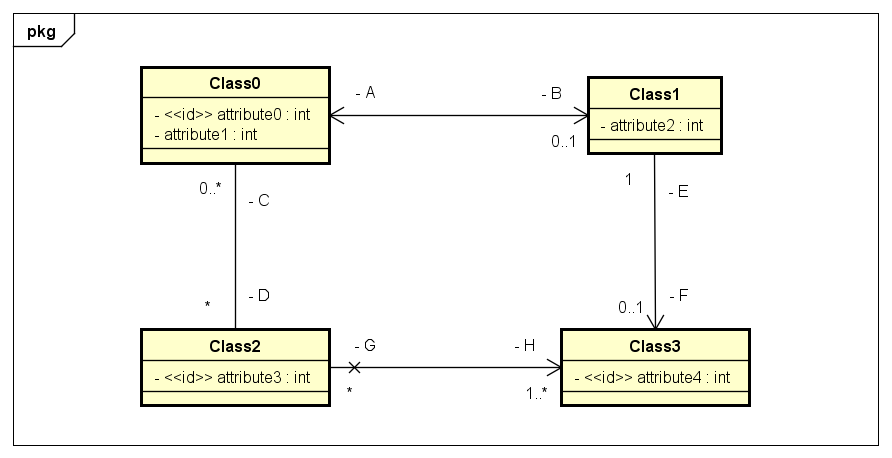
\includegraphics[scale=0.7]{imagens/Example_Multiplicity.png}
    \end{center}
	\caption{\label{fig_example_multiplicity}Exemplo de Diagrama de Classes UML com Associações Simples - Astah}
\end{figure}

A Figura \ref{fig_example_multiplicity} apresenta um exemplo de diversas possíveis aplicações de associações simples à um diagrama. O resultado da conversão deste diagrama é apresentado no Anexo \ref{fig_example_multiplicity_j}. A seguir é apresentada a aplicação das regras de conversão descritas até este ponto sobre o diagrama da Figura \ref{fig_example_multiplicity}:

\begin{itemize}
    \item Cada uma das classes tem um elemento criado em \textit{definitions}, conforme RCs 1-10.

    \item \textit{Class1} tem um atributo identificador criado, visto que não possui nenhum atributo anotado com o esteriótipo <<id>>, conforme RM02.

    \item \textit{Class0} tem adicionado as suas propriedades o atributo identificador de \textit{Class1} anotado como opcional, dado o vértice navegável B de multiplicidade 0..1, conforme RC13.

    \item \textit{Class0} tem adicionado as suas propriedades um vetor do atributo identificador de \textit{Class2} anotado como opcional, dado o vértice navegável D de multiplicidade *, conforme e RC14.

    \item \textit{Class1} tem adicionado as suas propriedades o atributo identificador de \textit{Class0} anotado como opcional, dado o vértice navegável A de multiplicidade não definida, conforme RM16 e RC13.

    \item \textit{Class1} tem adicionado as suas propriedades o atributo identificador de \textit{Class3} anotado como opcional, dado o vértice navegável F de multiplicidade 0..1, conforme RC13.

    \item \textit{Class2} tem adicionado as suas propriedades um vetor do atributo identificador de \textit{Class0} anotado como opcional, dado o vértice navegável C de multiplicidade 0..*, conforme RM15 e RC14.

    \item \textit{Class2} tem adicionado as suas propriedades um vetor do atributo identificador de \textit{Class3} com tamanho mínimo 1, dado o vértice navegável H de multiplicidade 1..*, conforme RC14.

    \item \textit{Class3} não tem adicionado as suas propriedades um vetor do atributo identificador de \textit{Class2}, dado o vértice não navegável G de multiplicidade *, conforme RMs 15 e 17.

    \item \textit{Class3} não tem adicionado as suas propriedades o atributo identificador de \textit{Class1}, dado o vértice de navegabilidade não definida E de multiplicidade 1, conforme RM 15.
\end{itemize}

%------------------------------------------------------------

\subsubsection{Associações de Generalização/Especialização}

Associações de Generalização/Especialização (Herança) permitem o reuso e a extensão de classes representadas no modelo de configuração. As restrições aplicadas a este tipo de associação são:

\begin{itemize}
    \item RM18: Uma classe pode ser uma Especialização de uma e apenas uma outra classe, não sendo permitida a modelagem de herança múltipla para fins desta ferramenta.

    \item RM19: Todas as associações de Generalização/Especialização são consideradas Parciais e Não-exclusivas. Isto se dá devido a complexidade de modelar estas características de forma explícita na ferramenta Astah.

    \item RM20: Uma classe ``filha'' não pode ter atributos identificadores, sendo estes necessariamente herdados da classe ``pai''.
\end{itemize}

É necessária uma única regra de conversão para que este tipo de associação seja contemplado:

\begin{itemize}
    \item RC15: A classe ``filha'' de uma associação de Realização/Especialização será representada na PFIS pela composição de seus atributos e uma referência à classe ``pai''.
\end{itemize}

A Figura \ref{fig_example_realization} apresenta um exemplo válido de diagrama de classes utilizando associações de Especialização/Generalização. O JSON Schema relacionado é apresentado no Anexo \ref{fig_example_realization_j}.

\begin{figure}
    \begin{center}
        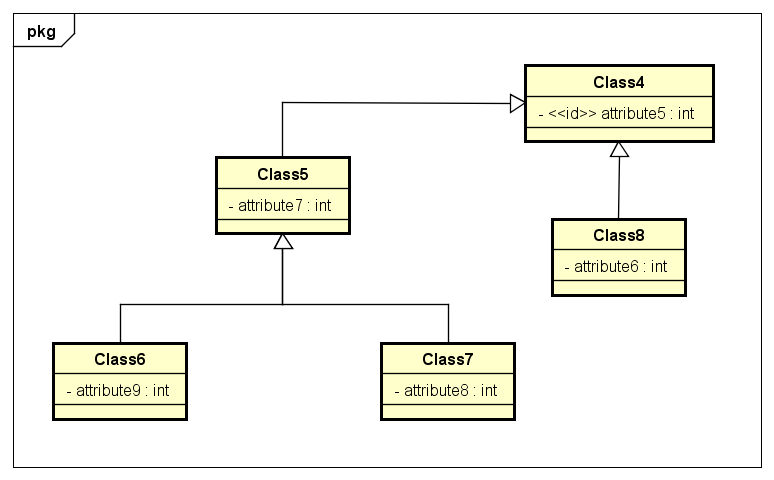
\includegraphics[scale=0.7]{imagens/Example_Realization.png}
    \end{center}
	\caption{\label{fig_example_realization}Exemplo de Diagrama de Classes UML com Associações de Generalização/Especialização - Astah}
\end{figure}

%------------------------------------------------------------

\subsubsection{Associações de Agregação}

Associações de Agregação permitem a representação de posse de uma classe sobre outra. Dois tipos de agregação são permitidos: Agregação Simples e Agregação por Composição. As restrições aplicadas a este tipo de associação são:

\begin{itemize}
    \item RM21: Associações de Agregação Simples representam a posse de uma classe sobre outra, porém mantendo a independência funcional de cada uma das classes associadas.

    \item RM22: Associações de Agregação por Composição representam a posse de uma classe sobre outra, sendo a classe ``possuída'' uma definição interna da classe ``possessora''. Desta forma, a classe possuída só pode existir no contexto da classe possessora.

    \item RM23: O vértice possuído de Associações de Agregação pode ter multiplicidade 1, 0..1, 0..*, * ou 1..*.

    \item RM24: O vértice possessor de Associações de Agregação deve ter multiplicidade 1.

    \item RM26: Não é comportada navegabilidade direcionada da classe possuída para a classe possessora, por limitação da notação gráfica da ferramenta Astah. Por esta razão, assume-se sempre navegabilidade unidirecional para associações de agregação.
\end{itemize}

São estabelecidas as seguintes regras de conversão para que este tipo de associação seja contemplado:

\begin{itemize}
    \item RC16: O vértice possuído de Associações de Agregação não será representado.

    \item RC17: O vértice possessor de Associações de Agregação Simples será representado por uma referência à classe possuída, ou um vetor de referências à classe possuída, definido de acordo com a multiplicidade do vetor, de forma similar a RCs 13-14.

    \item RC18: O vértice possessor de Associações de Agregação por Composição será representado por uma definição interna de classe, seguindo as regras de multiplicidade das RCs 13-14 para decisão de uso de definição única ou vetor.

    \item RC19: Classes possuídas de Associações de Agregação por Composição não serão representadas nas definições base.
\end{itemize}

A Figura \ref{fig_example_aggregation} apresenta um diagrama de classes que utiliza os dois tipos de associação de agregação, além de um tipo de associação simples para que seja possível visualizar a diferença entre estes. O Anexo \ref{fig_example_aggregation_j} apresenta o JSON Schema resultante da conversão deste diagrama.

\begin{figure}
    \begin{center}
        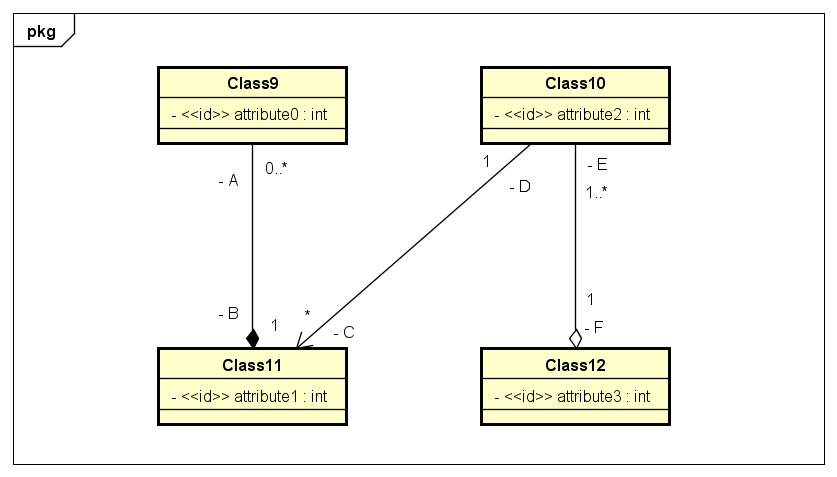
\includegraphics[scale=0.7]{imagens/Example_Aggregation.png}
    \end{center}
	\caption{\label{fig_example_aggregation}Exemplo de Diagrama de Classes UML com Associações de Agregação - Astah}
\end{figure}

%------------------------------------------------------------

\subsubsection{Classes Associativas}

Classes Associativas podem ser utilizadas para representar associações entre classes que contém atributos próprios. A seguinte restrição se aplica:

\begin{itemize}
    \item RM27: Classes Associativas não podem possuir atributo identificador; os identificadores das classes associadas são utilizados.
\end{itemize}

As regras de conversão referentes a esta restrição são:

\begin{itemize}
    \item RC20: Cada uma das classes associadas irá receber um vetor de referências à objetos da classe associativa.

    \item RC21: Um objeto será criado em \textit{definitions} para a classe associativa, utilizando como identificador a composição dos identificadores das classes associadas.
\end{itemize}

A Figura \ref{fig_example_association_class} apresenta um diagrama de classes exemplo. O Anexo \ref{fig_example_association_class_j} apresenta o JSON Schema resultante da conversão deste diagrama.

\begin{figure}
    \begin{center}
        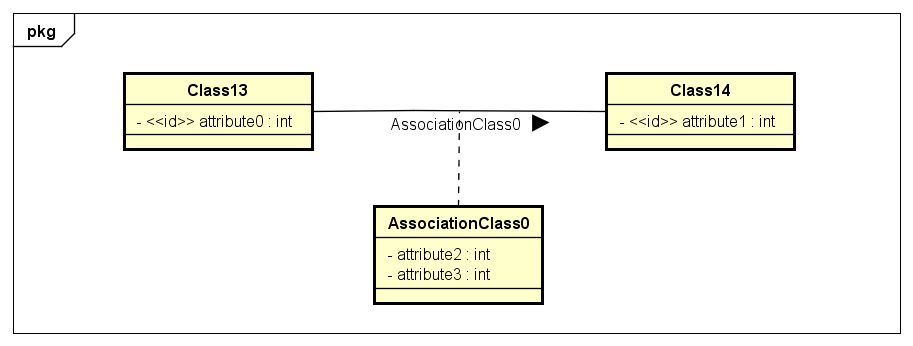
\includegraphics[scale=0.7]{imagens/Example_Association_Class.png}
    \end{center}
	\caption{\label{fig_example_association_class}Exemplo de Diagrama de Classes UML com Classe Associativa - Astah}
\end{figure}

%------------------------------------------------------------

%\subsection{Algoritmo de Geração de JSON Schema a partir de XML}

%A ferramenta AutoREST implementada como prova de conceito deste estudo irá utilizar um subconjunto dos elementos de Diagramas de Classes UML descritos em \cite{OMG:2011}, modelado na ferramenta Astah, para a criação de um arquivo JSON Schema de acordo com \citeonline{PEZOA:2016}. Este subconjunto e sua interpretação semântica na ferramenta AutoREST estão descritos a seguir, assim como as regras de modelagem que devem ser seguidas para que o diagrama seja válido como artefato de entrado do sistema AutoREST.

%\begin{itemize}
%    \item Classe: Representa um elemento do tipo \textit{object} em JSON Schema e uma \textit{collection} em MongoDB. Não possui restrições de nomenclatura.
%    \item Atributo de Classe: Representa uma propriedade da classe em JSON Schema. Atributos de Classe devem ser tipados corretamente como: int, representando o tipo JSON "integer"; float, representando "number"; string, ou; boolean. Para atributos que serão usados como chave primária, o nome deve ser escrito "\textless nome\textgreater \_id". Atributos usados como chave estrangeira serão sub-entendidos a partir dos relacionamentos utilizados. O caso particular de atributos do tipo "DateTime"\ devem ser tipados como float.
%    \item Associação: É entendida pelo sistema como representação de chaves estrangeiras, de acordo com a cardinalidade utilizada, da seguinte forma: para associações 0..*, a classe representada no ponto oposto da associação terá como chave estrangeira um vetor com as chaves primárias da classe representada no ponto 0..* da associação. Associações *..* terão chaves estrangeiras em ambos os pontos da associação. Associações 1..* terão como chave estrangeira a chave primária do ponto da associação 1, representado no ponto da associação *. Associações 1..1 não são suportadas. Todas as chaves estrangeiras criadas pelo sistema tem o formato "\textless nome\textgreater \_fk".
%    \item Associação de Composição: É entendida pelo sistema como representando, na classe "agregada", uma classe interna. É representada em JSON Schema utilizando o tipo de recurso "refSch".
%    \item Classe Associativa: É entendida pelo sistema como um "object"\ cuja chave primária é composta pelas chaves estrangeiras advindas das classes a que está associada. Estas chaves estrangeiras são representadas com a string "\textless nome\textgreater \_fk" e sub-entendidas pelo gerador de código como chave primária composta.
%\end{itemize}

%Além destas notações, o sistema AutoREST espera uma notação em formato de "tag"\ para algumas especificações de propriedades JSON. As tags aceitas pelo sistema são:

%\begin{itemize}
%    \item minLength: Específico para propriedades de tipo string, representa o tamanho mínimo da string. Deve ser anotado em formato numérico.
%    \item maxLength: Específico para propriedades de tipo string, representa o tamanho máximo da string. Deve ser anotado em formato numérico.
%    \item pattern: Específico para propriedades de tipo string, representa o padrão que deve ser seguido pela string. Deve ser anotado em formato de expressão regular.
%    \item minimum: Específico para propriedades de tipo integer e number, representa o valor mínimo da propriedade. Deve ser anotado em formato numérico.
%    \item maximum: Específico para propriedades de tipo integer e number, representa o valor máximo da propriedade. Deve ser anotado em formato numérico.
%    \item exclusiveMinimum: Específico para propriedades de tipo integer e number, classifica se o valor especificado como mínimo é inclusivo ou não. Deve ser representada com o valor booleano true ou false. Caso não esteja presente, assume-se como false.
%    \item exclusiveMaximum: Específico para propriedades de tipo integer e number, classifica se o valor especificado como máximo é inclusivo ou não. Deve ser representada com o valor booleano true ou false. Caso não esteja presente, assume-se como false.
%\end{itemize}

%O algoritmo utilizado para a conversão do formato XMI para o formato JSON Schema é descrito abaixo, em formato de pseudo-código.

%\begin{algorithm}
%\caption{Pseudo-código da tradução de XMI para JSON Schema}
%\begin{algorithmic}
%    \ForAll{Classes}
%        \State Create new JSON Schema object
%        \ForAll{Attributes}
%            \State Create new JSON Schema property
%            \If{Attribute has Tags}
%                \State Create appropriate restrictions
%            \EndIf
%        \EndFor
%    \EndFor
%
%    \ForAll{Associations}
%        \State Create appropriate foreign keys
%    \EndFor
%
%    \State Create definition block
%\end{algorithmic}
%\end{algorithm}

%------------------------------------------------------------

\subsection{Gramática BNF para Geração de Código a partir de JSON Schema}
\label{sec:bnf}

No trabalho de \citeonline{PEZOA:2016} é definida e validada formalmente uma gramática na forma de Backus-Naur (BNF) para a estrutura JSON Schema \cite{GALIEGUE:2013}. Nesta seção, serão exploradas as partes desta gramática utilizadas no subsistema \textit{REST API Generator} e seu significado semântico.

%------------------------------------------------------------

\subsubsection{Sintaxe}
A gramática BNF foi usada como entrada para a geração de um \textit{parser} na ferramenta BYACC/J \cite{BYACCJ}. O subconjunto de definições que serão relevantes para o subsistema está contido na definição \textit{defs}, que corresponde à propriedade \textit{definitions} de um JSON Schema. Cada \textit{defs} possui no mínimo um \textit{kSch}, que é composto de um nome (\textit{kword}) e uma ou mais restrições (\textit{res}). Conforme segmento extraído de \cite{PEZOA:2016}:

\begin{algorithmic}
    \item \textbf{defs} := ``definitions'': \{ \textbf{kSch} (, \textbf{kSch})*\}
    \item \textbf{kSch} := \textbf{kword}: \{ \textbf{JSch} \}
    \item \textbf{JSch} := ( \textbf{res} (, \textbf{res})*)
    \item \textbf{res} := \textbf{type} | \textbf{strRes} | \textbf{numRes} | \textbf{arrRes} | \textbf{objRes} | \textbf{multRes} | \textbf{refSch} | \textbf{title} | \textbf{description}
\end{algorithmic}

A gramática utilizada serve para a validação sintática completa de um JSON Schema; porém somente algumas das definições terão significado semântico para o subsistema, conforme seção a seguir. A gramática completa está no Anexo \ref{anexo:bnfjs}.

\subsubsection{Semântica}

Nesta seção, serão apresentadas as derivações \textit{kSch}, que deriva de \textit{defs}, consideradas no processo de criação da API REST, assim como suas derivações utilizadas. Em sequência, serão apresentados os processos de geração do código fonte final, subseções \ref{sec:bnf:http} e \ref{sec:bnf:mongo}.

%Todas as 'definitions' devem estar no primeiro nivel e somente serem referenciadas referenciadas nos niveis abaixo
%Verificar termos abaixo desta derivação que serão ignorados, por nao se aplicarão a nossa ferramenta, candicados possiveis sao as restrições de multiplicidade

\subsubsubsection{Derivações de \textit{kSch}}
\label{sec:bnf:ksch}

Cada \textit{kSch} será considerada a definição de um \textit{resource} a ser fornecido pela API. Logo, a derivação \textit{kword} se tornará o nome deste \textit{resource}. A derivação \textit{JSch} será utilizada para a geração de métodos HTTP disponibilizados para o \textit{resource}, assim como para a criação de um \textit{model} do módulo Mongoose de Node.js, que subsequentemente irá fazer as interações com o MongoDB. As derivações utilizadas para um \textit{JSch} de um \textit{resource} são:
\begin{itemize}
    %\item \textbf{title}: título do \textit{resource}

    %\item \textbf{description}: descrição do \textit{resource}

    \item \textbf{type}: restringe o tipo do objeto sendo definido. Para um \textit{resource} o valor deverá ser \textit{object}; outros valores serão considerados inválidos
    %\item \textbf{strRes}: restrições aplicáveis a \textit{strings}
    %\item \textbf{numRes}: restrições aplicáveis a números (inteiros e decimais)
    %\item \textbf{arrRes}: restrições a \textit{arrays}

    \item \textbf{objRes}: restrições do \textit{resource}; serão consideradas as definições na Subseção \ref{sec:bnf:obj}
    %\item \textbf{multRes}: restrições de multiplicidade, enumerações, conjunções e disjunções
    %\item \textbf{refSch}: referências a outros \textit{schemas}, seja localmente ou em outro arquivo
\end{itemize}

\subsubsubsection{Derivações de \textit{objRes}}
\label{sec:bnf:obj}
A diretiva \textit{objRes} representa as restrições relacionadas a definição de um objeto. Ela pode ser usada tanto para definição de \textit{resources} quanto para a definição de propriedades do tipo objeto. As derivações consideradas válidas são as seguintes:

\begin{itemize}
    \item \textbf{properties}: irá conter as propriedades do objeto sendo definido; será melhor detalhada na Seção \ref{sec:bnf:props}.

    %\item \textbf{additionalProperties}: indica se o objeto poderá conter propriedades adicionais, para esta derivação é esperado somente um valor booleano (\textit{true} ou \textit{false}), outros valores serão considerados inválidos

    \item \textbf{required}: define quais propriedades são obrigatórias

    \item \textbf{dependencies}: será considerada nesta diretiva somente a derivação contendo um \textit{kArr}, que é o nome de uma propriedade e suas dependências. Todas as propriedades serão dependentes da propriedade definida como chave primária, para que a chave primária seja composta será necessario que as propriedades sejam dependentes de mais de uma propriedade
\end{itemize}

\subsubsubsection{Derivações de \textit{properties}}
\label{sec:bnf:props}
As propriedades de um objeto serão todas as derivações \textit{kSch} que fazem parte da diretiva \textit{properties} relacionada ao mesmo. Porém, as derivações de um \textit{kSch} terão um significado diferente quando aplicadas a uma propriedade do que quanto aplicadas a um \textit{resource}. A derivação \textit{kword} será o nome da propriedade e para a derivação \textit{JSch} serão consideradas válidas somente as derivações listadas a seguir:
\begin{itemize}
    %\item \textbf{title}: título da propriedade

    %\item \textbf{description}: descrição da propriedade

    \item \textbf{type}: restringe o tipo da propriedade sendo definida. Caso nenhum valor seja informado assume-se \textit{object}. Valores considerados válidos são: \textit{string}, \textit{integer}, \textit{number}, \textit{boolean}, \textit{object} e \textit{array}.

    \item \textbf{strRes}: será aceita quando o \textit{type} for \textit{string} e serão consideradas válidas as seguintes derivações:
    \begin{itemize}
        \item \textbf{minLength}: tamanho mínimo do valor da propriedade
        \item \textbf{maxLength}: tamanho máximo do valor da propriedade
        \item \textbf{pattern}: expressão regular para validação do valor\footnote{Esta funcionalidade apesar de especificada, não está presente na ferramenta prova de conceito}
    \end{itemize}

    \item \textbf{numRes}: será aceita quando o \textit{type} for \textit{integer} ou \textit{number} e serão consideradas válidas as seguintes derivações:
    \begin{itemize}
        \item \textbf{minimum}: valor mínimo da propriedade
        \item \textbf{exclusiveMinimum}: valor booleano. Indica se o valor mínimo está incluído ou não no intervalo de validação
        \item \textbf{maximum}: valor máximo da propriedade
        \item \textbf{exclusiveMaximum}: valor booleano. Indica se o valor máximo está incluído ou não no intervalo de validação
    \end{itemize}

    \item \textbf{arrRes}: será aceita quando o \textit{type} for \textit{array}, será melhor detalhada na Subseção \ref{sec:bnf:arr}

    \item \textbf{objRes}: será aceita quando o \textit{type} for \textit{object}. Serão aplicadas as definições da Subseção \ref{sec:bnf:obj}
    %\item \textbf{multRes}: restrições de multiplicidade, enumerações, conjunções e disjunções

    \item \textbf{refSch}: referências a outras definições no arquivo JSON Schema que está sendo processado. Eestas referências possuirão significados diferentes, de acordo com seu contexto, na disponibilização dos \textit{resources} pela API, conforme Seções \ref{sec:bnf:mongo} e \ref{sec:bnf:http}
\end{itemize}

\subsubsubsection{Derivações de \textit{arrRes}}
\label{sec:bnf:arr}
As restrições desta diretiva são relacionadas ao \textit{type array}. Serão aceitas as seguintes derivações:
\begin{itemize}
    \item \textbf{items}: definição dos tipos do \textit{array}. Pode ser derivada de duas formas:
    \begin{itemize}
        \item \textbf{sameitems}: determina que todos os itens do \textit{array} possuem a mesma definição, que é determinada por um \textit{JSch}. Para esta definição são aceitas as mesmas derivações de \textit{JSch} da Subseção \ref{sec:bnf:props}

        \item \textbf{varitems}: determina que o \textit{array} pode ter itens de definições variadas. Esta derivação é considerada inválida pelo gerador

    \end{itemize}

    %\item \textbf{additems}: é uma derivação que espera um valor booleano e opcional pois

    \item \textbf{minitems}: indica o numero mínimo de itens do \textit{array}

    \item \textbf{maxitems}: indica o numero máximo de itens do \textit{array}
\end{itemize}


\subsubsubsection{Geração dos \textit{models} Mongoose}
\label{sec:bnf:mongo}

Para a criação dos \textit{models} de cada \textit{resource} são usadas as seguintes regras de criação:
\begin{itemize}
    \item Cada propriedade do \textit{resource} no JSON Schema irá resultar em uma propriedade do \textit{model} Mongoose

    \item Uma propriedade do tipo \textit{integer} no JSON Schema resultará em uma propriedade Mongoose com propriedades \textit{type: Number} e \textit{integer: true}

    \item Uma propriedade do tipo \textit{number} no JSON Schema resultará em uma propriedade Mongoose com a propriedade \textit{type: Number}

    \item Uma propriedade do tipo \textit{boolean} no JSON Schema resultará em uma propriedade Mongoose com a propriedade \textit{type: Boolean}

    \item Uma propriedade do tipo \textit{string} no JSON Schema resultará em uma propriedade Mongoose com a propriedade \textit{type: String}

    \item Uma propriedade do tipo \textit{array} no JSON Schema resultará em uma propriedade Mongoose com uma propriedade \textit{any} que será um \textit{array} contendo o \textit{SchemaType} Mongoose dos elementos

    \item Uma propriedade do tipo \textit{object} no JSON Schema resultará em uma propriedade Mongoose com a propriedade \textit{type: Object}. Se esta propriedade \textit{object} possuir definições JSON Schema, esta serão criadas no Mongoose conforme estas mesmas regras

    \item Todas as propriedades do JSON Schema especificadas como \textit{required} receberão uma propriedade Mongoose \textit{required: true}

    \item Todas as propriedades do JSON Schema dos tipos \textit{number} e \textit{integer} que possuírem definições de máximo e mínimo receberão propriedades Mongoose correspondentes

    \item Propriedades do JSON Schema do tipo \textit{string} que possuírem definições de tamanho máximo, tamanho mínimo e expressão regular receberão propriedades Mongoose correspondentes\footnote{Esta funcionalidade apesar de especificada, não está presente na ferramenta prova de conceito}

\end{itemize}

As definições \textit{dependencies} do JSON Schema são interpretadas como se referindo a chave primária de um \textit{resource}. Logo, a propriedade da qual todas as outras dependem será considerada a chave primária. O MongoDB considera como chave primária de suas \textit{collections} a propriedade \textit{\_id} e este comportamento é assimilado pelo Mongoose.

Se for identificado que um \textit{resource} possui uma chave primária composta por mais de uma propriedade, ele receberá um \textit{index unique} que contenha todas estas propriedades que compõem a chave, fazendo-o assim respeitar a restrição de unicidade da chave primária.

Para \textit{arrays} e propriedades que possuam referências (\textbf{refSch}) a outros \textit{resources}, a criação do \textit{model} sofrerá alterações. Se um \textit{array} possuir itens que são referências (\textbf{refSch}) a outro \textit{resource}, então o que será armazenado no MongoDB serão os valores das chaves primárias deste \textit{resource}, e o \textit{model} Mongoose possuirá propriedades correspondentes. Quando uma propriedade for referência a outro \textit{resource} isto implicará em uma herança. Neste caso o \textit{model} que contém esta propriedade será armazenado na mesma \textit{collection} no MongoDB e possuirá seu \textit{Schema} de Mongoose representando o relacionamento de herança.

Para que os \textit{resources} fornecidos pela API não contenham propriedades não desejadas, e ainda seja possível utilizar a chave primária com seu nome original, serão utilizados métodos de acesso virtuais do Mongoose. Como exemplo temos no Listing \ref{lst_virtual} o atributo \textit{attribute0} da classe apresentada na Figura \ref{fig_example_class}. O código completo para o \textit{model} desta classe está no Anexo \ref{anexo:model_mongoose}.

\begin{listing}
\begin{minted}[frame=single,
                framesep=3mm,
                linenos=true,
                xleftmargin=21pt,
                breaklines=true,
                tabsize=4]{js}
Example_ClassSchema.virtual('attribute0').get(function() {
    return this._id;
});
Example_ClassSchema.virtual('attribute0').set(function (value) {
    this._id = value;
});
\end{minted}
\caption{Exemplo métodos virtuais Mongoose}
\label{lst_virtual}
\end{listing}

Além da propriedade \textit{\_id} do MongoDB, o Mongoose também adiciona outras propriedades que não estariam de acordo com o JSON Schema do \textit{resource}. Para evitar o envio destas propriedades, todos os \textit{models} possuirão o método \textit{cleanObject}, que terá a função de retornar um objeto sem estas propriedades. Um exemplo aplicado a classe \textit{Example\_Class} pode ser visto no Listing \ref{lst_clean_obj}.

\begin{listing}
\begin{minted}[frame=single,
                framesep=3mm,
                linenos=true,
                xleftmargin=21pt,
                breaklines=true,
                tabsize=4]{js}
Example_ClassSchema.methods.cleanObject = function() {
    var doc = this.toObject({ virtuals: true });
    delete doc.__v;
    delete doc._id;
    delete doc.id;
    return doc;
};
\end{minted}
\caption{Exemplo método \textit{cleanObject}}
\label{lst_clean_obj}
\end{listing}

\subsubsubsection{Geração dos métodos HTTP}
\label{sec:bnf:http}

Cada \textit{resource} terá seus métodos HTTP dentro de um \textit{middleware} do tipo \textit{Router}, que será utilizado pelo módulo \textit{Express} do \textit{Node.js} para gerenciar as \textit{requests}.

Os métodos HTTP gerados para um \textit{resource} serão todos os identificados como necessários para realizar as operações CRUD, que são: GET, HEAD, POST, PUT, PATCH e DELETE.

Um \textit{resource} com uma chave primária simples possuirá os \textit{endpoints} apresentados na Tabela \ref{tab:http_1}, onde: \textit{resourceName} é o nome do \textit{resource}, e; \textit{identifier} é a chave primária do resource. As \textit{query strings} nas URIs indicadas são opcionais e os parâmetros esperados seriam \textit{propName}, que é o nome de uma propriedade, e \textit{valueX}, que é o valor desejado na propriedade; é possível mais de um parâmetro de filtro na \textit{query string}.

\begin{table}[]
    \centering
    \begin{tabularx}{\textwidth}{|l|l|X|}
        \hline
        \textbf{Método} & \textbf{URI} & \textbf{Função} \\
        \hline

        GET & /resourceName/[?propName=valueX]            & Retornar todos os \textit{resources} da \textit{collection}\\
        \hline

        GET & /resourceName/:identifier & Retornar o \textit{resource} com o \textit{identifier} igual ao parâmetro na URI\\
        \hline

        HEAD & /resourceName/:identifier & Verificar se o \textit{resource} com o \textit{identifier} igual ao parâmetro indicado existe, sem retorná-lo\\
        \hline

        POST & /resourceName/ & Inserir ou modificar totalmente o \textit{resource} contido no \textit{message body} da \textit{request}\\
        \hline

        PUT & /resourceName/:identifier & Inserir ou modificar totalmente o \textit{resource} indicado pelo parâmetro da URI, utilizando os dados contidos no \textit{message body} da \textit{request}\\
        \hline

        PATCH & /resourceName/:identifier & Modificar parcialmente o \textit{resource} indicado pelo parâmetro da URI, utilizando os dados contidos no \textit{message body} da \textit{request}\\
        \hline

        DELETE & /resourceName/:identifier & Excluir o \textit{resource} com o \textit{identifier} igual ao parâmetro indicado\\
        \hline
    \end{tabularx}
    \caption{\textit{Resource} Simples - Métodos HTTP e URIs}
    \label{tab:http_1}
\end{table}

Se um \textit{resource} possuir uma chave composta, seus \textit{endpoints} ao invés de aceitarem um \textit{identifier} irão esperar que os valores das chaves sejam enviados via \textit{query string}; e o comportamento gerado para o caso de nem todas as chaves serem enviadas na \textit{query string} será de um erro retornado ao cliente. Estas alterações nos \textit{endpoints} são apresentadas na Tabela \ref{tab:http_2}; a função dos métodos permanecem as mesmas.

\begin{table}[]
    \centering
    \begin{tabularx}{\textwidth}{|l|l|X|}
        \hline
        \textbf{Método} & \textbf{URI} & \textbf{\textit{Query string}} \\
        \hline

        GET & /resourceName/[?propName=valueX] & Opcional, utilizado somente para filtro, aplicável a todas as propriedades\\
        \hline

        HEAD & /resourceName/[?propName=valueX] & Devem ser informados os valores da chave primária\\
        \hline

        POST & /resourceName/ & Não aplicável (mantém comportamento utilizando o \textit{message body})\\
        \hline

        PUT & /resourceName/[?propName=valueX] & Devem ser informados os valores da chave primária\\
        \hline

        PATCH & /resourceName/[?propName=valueX] & Devem ser informados os valores da chave primária\\
        \hline

        DELETE & /resourceName/[?propName=valueX] & Devem ser informados os valores da chave primária\\
        \hline
    \end{tabularx}
    \caption{\textit{Resource} com chave composta - Métodos HTTP e URIs}
    \label{tab:http_2}
\end{table}

Quando um \textit{resource} com chave primária simples possuir propriedades complexas ou do tipo \textit{array}, estas poderão ser acessadas diretamente através de \textit{endpoints} dedicados a elas se o \textit{endpoint} já possuir o \textit{identifier} do \textit{resource}. Estes \textit{endpoints} serão formados utilizando o \textit{endpoint} do \textit{resource} e um sufixo com o nome da propriedade, conforme Tabela \ref{tab:end_prop}. Propriedades complexas que estão contidas dentro de outras propriedades complexas possuirão seus \textit{endpoints} também, sendo estes criados com o mesmo procedimento: adicionando um sufixo com o nome da propriedade aos \textit{endpoints} já existentes.

\begin{table}[]
    \centering
    \begin{tabularx}{\textwidth}{|l|l|X|}
        \hline
        \textbf{Método} & \textbf{URI} & \textbf{\textit{Query string}} \\
        \hline

        GET & /resourceName/:identifier/propName & Retornar o conteúdo da propriedade \textit{propName} do \textit{resource} com o \textit{identifier} igual ao parâmetro na URI\\
        \hline

        HEAD & /resourceName/:identifier/propName & Verificar se o \textit{resource} com o \textit{identifier} igual ao parâmetro indicado existe e possui a propriedade \textit{propName}, sem retornar seu valor\\
        \hline

        PUT & /resourceName/:identifier/propName & Inserir ou modificar totalmente o conteúdo da propriedade \textit{propName} no \textit{resource} indicado pelo parâmetro da URI, utilizando os dados contidos no \textit{message body} da \textit{request}\\
        \hline

        PATCH & /resourceName/:identifier/propName & Modificar parcialmente o conteúdo da propriedade \textit{propName} do \textit{resource} indicado pelo parâmetro da URI, utilizando os dados contidos no \textit{message body} da \textit{request}. Não aplicável a propriedades \textit{array}\\
        \hline

        DELETE & /resourceName/:identifier/propName & Excluir a propriedade \textit{propName} do \textit{resource} com o \textit{identifier} igual ao parâmetro indicado\\
        \hline
        \hline
    \end{tabularx}
    \caption{\textit{Endpoints} de propriedades complexas e \textit{arrays}}
    \label{tab:end_prop}
\end{table}

%A API gerada irá possuir ... status codes


\subsection{Funcionamento da API REST gerada}

A API gerada poderá ser utilizada através de um arquivo ``\textit{api.js}''\ que será gerado após todos os \textit{models} e \textit{routers} serem gerados. Neste arquivo, o servidor \textit{Express} será criado e iniciado e os \textit{routers} gerados serão adicionados como \textit{middleware} do servidor. Também constarão no arquivo a criação da conexão com o MongoDB e outras utilidades que permitam uma melhor utilização dos recursos da linguagem.

Ao final da geração da API, é possivel utilizá-la através do arquivo \textit{api.js}, usando-o como parâmetro do \textit{runtime} de Node.js em um terminal e estando na pasta onde o arquivo se encontra; por exemplo: \textbf{node api.js}

Após executar este comando o usuário será informado de que a API está executando e também os \textit{endpoints} de GET de cada \textit{resource}, conforme exemplo da Figura \ref{fig:api_console}.

\begin{figure}
    \begin{center}
        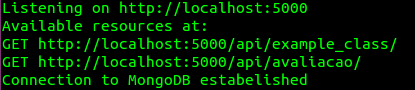
\includegraphics[scale=0.7]{imagens/outApiConsole.png}
    \end{center}
	\caption{\label{fig:api_console}Exemplo de servidor de API iniciado}
\end{figure}

O servidor \textit{Express} criado irá processar as \textit{requests} que forem recebidas, irá identificar a URI solicitada e o método HTTP e então irá encaminhar a \textit{request} para o \textit{router middleware} que, por sua vez, irá processar a \textit{request} e realizar a operação CRUD correspondente utilizando seu(s) respectivo(s) \textit{model(s)}. Esta sequência de processamento é mostrada no diagrama de sequências nas Figuras \ref{fig:seq_api_1} e \ref{fig:seq_api_2}.


\begin{figure}
    \begin{center}
        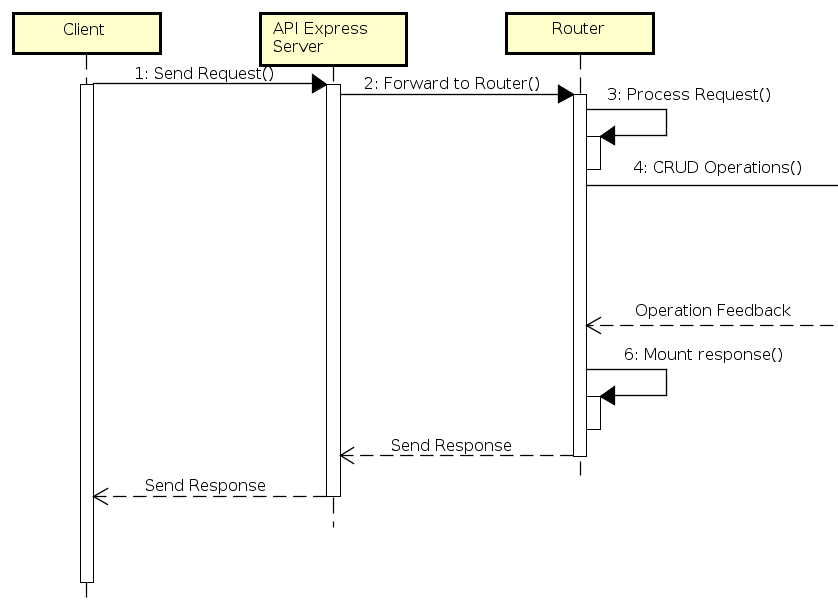
\includegraphics[scale=0.7]{imagens/API_Sequence_Diagram_1.png}
    \end{center}
	\caption{\label{fig:seq_api_1}Exemplo de processamento de \textit{request} no servidor da API - Parte 1}
\end{figure}

\begin{figure}
    \begin{center}
        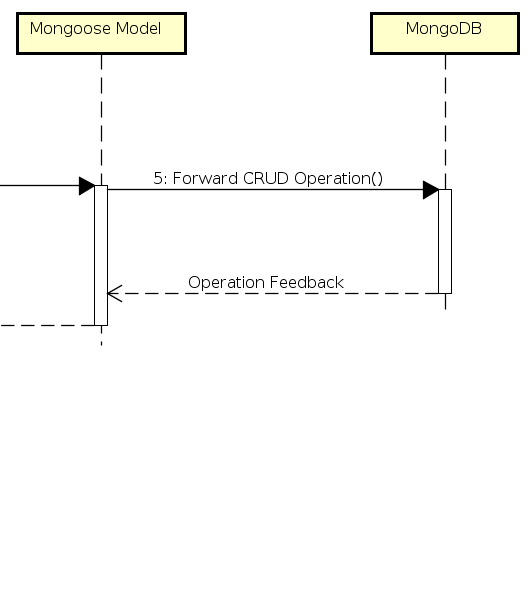
\includegraphics[scale=0.7]{imagens/API_Sequence_Diagram_2.png}
    \end{center}
	\caption{\label{fig:seq_api_2}Exemplo de processamento de \textit{request} no servidor da API - Parte 2}
\end{figure}

\subsection{Demonstração de resultados}
\label{sec:demo}

Para demonstrar a instanciação da solução AutoREST, uma aplicação \textit{web}, disponível no endereço \url{https://autorest-site.herokuapp.com/}, foi criada para a geração de APIs usando os componentes AutoREST, que são os seguintes:

\begin{itemize}
    \item \textit{\textbf{astah-xml-parser\footnote{\url{https://github.com/AutoREST/astah-xml-parser}}}}: responsável por realizar a conversão de XMLs em JSON Schemas. Também tem a funcionalidade de extrair os pacotes presentes no XML, para que seja possível a escolha de qual pacote contém as informações sobre a qual a API deve ser gerada;
    \item \textit{\textbf{rest-api-generator\footnote{\url{https://github.com/AutoREST/rest-api-generator}}}}: responsável por gerar as APIs usando um JSON Schema e algumas opções informadas na interface com o usuário;
    \item \textit{\textbf{autorest-site\footnote{\url{https://github.com/AutoREST/autorest-site}}}}: aplicação \textit{web} responsável por receber o arquivo de entrada para geração e algumas opções adicionais.
\end{itemize}

A interface com o usuário tem duas telas principais que são baseadas nos \textit{mockups} das Figuras \ref{fig:mindex} e \ref{fig:mpacks}. Na tela da Figura \ref{fig:mindex}, temos a entrada básica para a geração da API, onde:

\begin{figure}
    \begin{center}
        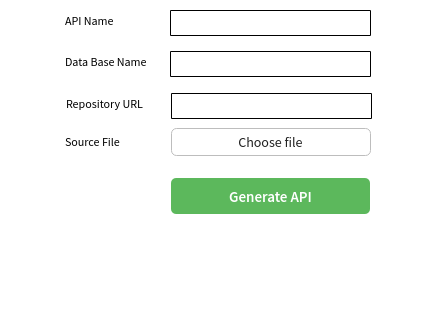
\includegraphics[scale=0.7]{imagens/Mockup_index.png}
    \end{center}
	\caption{\label{fig:mindex}Tela de entrada de dados para geração de API}
\end{figure}

\begin{figure}
    \begin{center}
        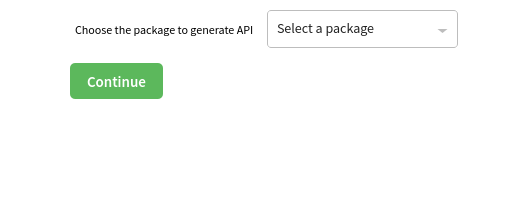
\includegraphics[scale=0.7]{imagens/Mockup_pack_select.png}
    \end{center}
	\caption{\label{fig:mpacks}Tela para seleção de \textit{package} da API}
\end{figure}

\begin{itemize}
    \item \textit{API Name}: é o nome da API; é usado para dar um nome em alguns pontos da API, assim como no arquivo de retorno final;
    \item \textit{Data Base Name}: nome do banco de dados usado na conexão com o MongoDB;
    \item \textit{Respository URL}: a URL onde a API será guardada; é somente para fins de documentação no \textit{package.json} da API;
    \item \textit{Source File}: arquivo contendo a especificação da API; aceita-se um XML da ferramenta Astah modelado conforme as regras de modelagem AutoREST ou um arquivo JSON Schema com restrições aceitas e coerentes com as regras de sintaxe e semântica AutoREST
    \item \textit{Generate API}: botão que inicia a geração da API
\end{itemize}

Caso o \textit{Source File} seja um XML que contenha mais de um \textit{package} de classes, o componente \textit{astah-xml-parser} irá retornar a lista de \textit{packages} disponíveis para que o usuário escolha qual deve ser a fonte de sua API; este é o comportamento apresentado na tela da Figura \ref{fig:mpacks}.

%end Demonstração de resultados
